\documentclass{ethpresentation}

\title{Building a 25 MHz NMR Spectrometer}
\date{\today}
\author{Maximilian Stabel}
\institute{ETH Zürich}

\begin{document}
  \maketitle
  % \section{First Section}
  \begin{frame}{Since last time}
    \begin{columns}
      \begin{column}{0.45\textwidth}
        \begin{itemize}
          \item Meeting with Christian Vogt
          \item Finished building probe
          \item Tune \& Match probe
          \item Explored measurement setup
          \item Thought about power supply
        \end{itemize}
      \end{column}
      \begin{column}{0.45\textwidth}
        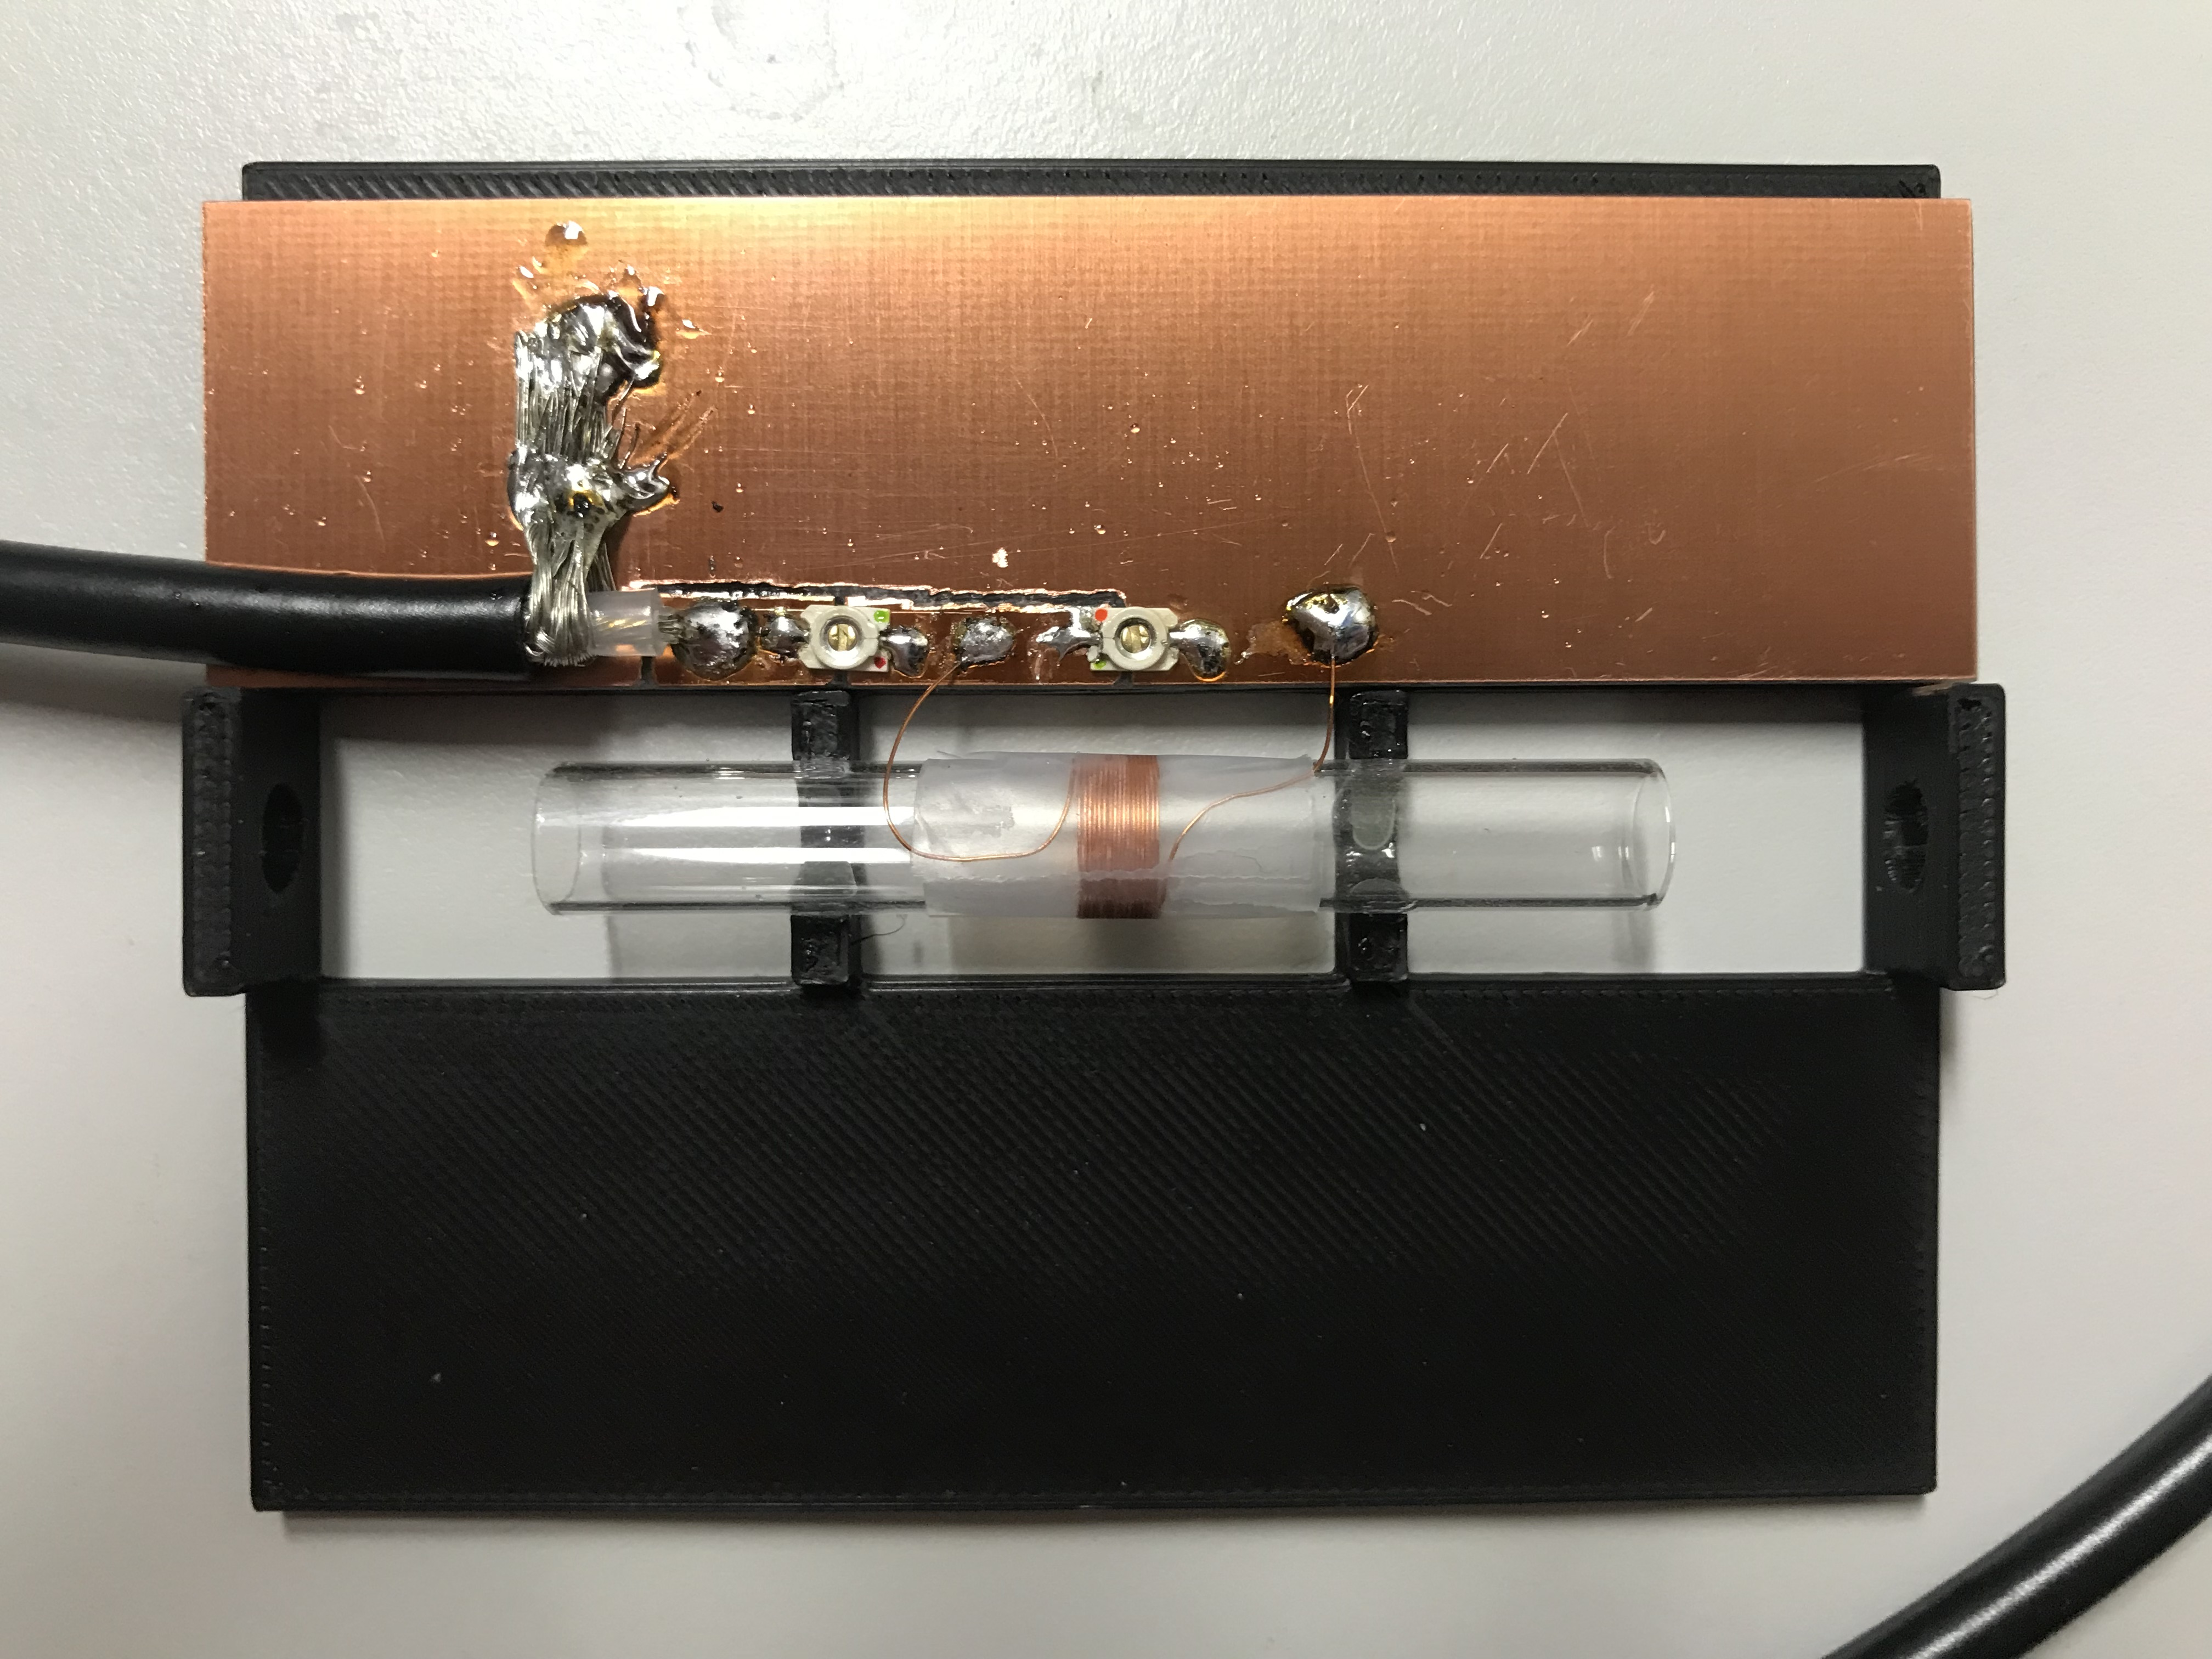
\includegraphics[width=\textwidth]{./img/230418-finished_probe_only.JPG}
      \end{column}
    \end{columns}
  \end{frame}
  \begin{frame}{Upcoming}
    \begin{itemize}
      \item Setup/Assemble spectrometer
      \item Measure water with probe v1
      \item Come up with single channel design for current source
      \item Simulate single channel
    \end{itemize}
  \end{frame}

  % \begin{frame}[standout]
  %   Thank you!
  % \end{frame}

  % \appendix
  % \begin{frame}[standout]
  %   A backup graph for explaining things.
  % \end{frame}
\end{document}